\apendice{Documentación de usuario}

\section{Introducción}
En este apartado se muestra el manual de usuario.\\
En su mayoría las imágenes o capturas, corresponden a la versión 1.0 de la aplicación, puede haber pequeños cambios visuales en la aplicación. En caso de un cambio mayor se habrá actualizado el manual.
\section{Requisitos de usuarios}
HealthApp no requiere de grandes requisitos. Exclusivamente, tener el ejecutable y un ordenador desde el cual ejecutarlo.
\section{Instalación}
La aplicación no requiere instalación, es una versión portable. Para su uso, descargue la aplicación del siguiente enlace: ENLACE\\
Una vez descargada descomprima el archivo , pulse el botón derecho del ratón y escoja la opción: "extraer aqui..."
\imagen{extraerApp}{Descomprimir el archivo ".zip" de la aplicación}
Una vez descomprimido iremos a la carpeta del proyecto y buscaremos el archivo \textbf{HealthApp.exe}
\imagen{ejecutable}{Localización del ejecutable del programa.}
Una vez localizado, haremos doble click izquierdo sobre el archivo para iniciar el programa. \textbf{Recomendación:} Crear un acceso directo al escritorio para mayor comodidad, para ello: Haga click derecho sobre HealthApp.exe, ''crear acceso directo''. Sitúe el acceso directo donde lo desee. A partir de ahora podrá ejecutar directamente el acceso directo.

\section{Manual del usuario}
\subsection{Inicio}
\begin{figure}[htb]
\centering
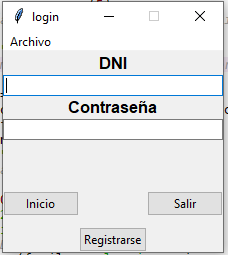
\includegraphics[scale=1]{Inicio} 
\caption{Pantalla de inicio del programa (Versión 2.0)}
\end{figure}
\subsubsection{Crear un Usuario/Registrarse}
Una vez abierto el programa, haga clic en el botón de \textbf{“Registrarse”}. 
\begin{figure}[htb]
\centering
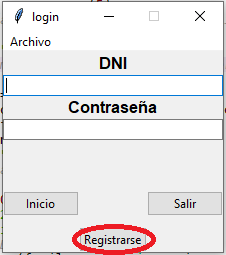
\includegraphics[scale=1]{inicioregistro} 
\caption{Pantalla de inicio, botón Registrar (Versión 1.0)}
\end{figure}

\begin{itemize}
\item	\textbf{DNI:} escriba su número del documento de DNI sin la letra, el cual será su usuario para iniciar sesión posteriormente. Ej: 71257992
\item	\textbf{Nombre:} escriba su nombre solo con letras, sin símbolos o signos.
\item	\textbf{Apellido:} escriba su nombre solo con letras, sin símbolos o signos.
\item	\textbf{Contraseña:} escriba la contraseña que quiere para iniciar sesión en la aplicación, sin límite de caracteres y/o símbolos.
\item	\textbf{Sexo:} marque su sexo haciendo clic encima del correspondiente.
\item	\textbf{Edad:} escriba su edad en números, sin letras o símbolos.
\item	\textbf{Altura:} escriba su altura en centímetros en números, sin letras o símbolos.
\item	\textbf{Peso:} escriba su peso en kilogramos en números, pudiendo incluir comas y decimales, pero no letras. Ej: 65,8
\item	\textbf{Actividad:} marque haciendo clic encima del número correspondiente al nivel de actividad que suele realizar. El significado de cada uno es:
\begin{itemize}
\item	1 - poco o ningún ejercicio.
\item	2 - ejercicio ligero (de 1 a 3 días por semana).
\item	3 - ejercicio moderado (de 3 a 5 días por semana).
\item	4 - ejercicio fuerte (6 días por semana).
\item	5 - ejercicio profesional o extremo.
\end{itemize}
\item	\textbf{Patología:} haga clic en el desplegable y seleccione si sufre alguna de las patologías sugeridas o “sin patología” en el caso de que no sea así.
\item	\textbf{Tipo:} marque haciendo clic encima del tipo de dieta que quiere, siendo:
\begin{itemize}
\item	Bajar - una dieta para bajar de peso de forma saludable.
\item	Mantener - una dieta para mantener el peso de forma saludable.
\item	Subir - una dieta para subir de peso de forma saludable.
\end{itemize}
\end{itemize}

Cuando haya rellenado todos los datos, pulse en el botón de “Aceptar y Guardar” para crear el usuario y guardar todos los datos que ha registrado (si falta algún campo por completar el programa dará error y no le permitirá guardar los cambios).
Se abrirá la siguiente ventana con los datos que deberá rellenar:
\imagen{registroguardar}{Ventana de registro del nuevo usuario señalizada para el registro (Version 1.0)}
También puede pulsar el botón de “Cancelar” si quiere salir cancelar el registro, o la “X” de la esquina de arriba a la derecha si desea cerrar la ventana.
\imagen{registrocerrar}{Ventana de registro del nuevo usuario señalizada para el cierre (Version 1.0)}
\subsubsection{INICIAR SESIÓN}
\imagen{LoginDetallado}{Inicio de sesión detallado (Versión 2.0)}
Para iniciar sesión en el programa con su usuario, escriba su DNI sin letra en el apartado llamado “DNI” (el cual será su número de usuario) y la contraseña que ha elegido anteriormente en la casilla denominada “Contraseña”. Cuando ya estén los dos campos rellenos con sus datos de usuario, pulse el botón de \textbf{''Inicio''} para iniciar el programa. Además, podrá encontrar el Manual de Usuario del programa en todo momento en la pestaña \textbf{``Archivo''}\\
Sino ha creado aún su usuario, acuda al apartado anterior del manual para seguir las instrucciones y registrarse.\\
Si desea salir o cerrar el programa, pulse el botón de “Salir” o la “X” de la esquina de arriba a la derecha.
\begin{figure}[htb]
\centering
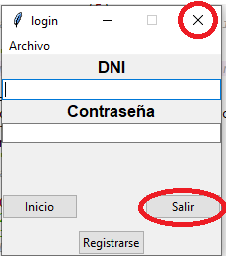
\includegraphics[scale=1]{InicioSalir} 
\caption{Imagen detallando el cierre del programa (Version 2.0}
\end{figure}

\subsection{PÁGINA PRINCIPAL}
\imagen{PagPrincipal}{Página principal de la aplicación (Version 1.0)}
\subsubsection{ARCHIVO}
\imagen{PPArchivo}{Pantalla Principal señalizando la opción Archivo (Versión 1.0)}
Arriba a la izquierda de la página encontrará el botón “Archivo”, en el que si pulsa se desplegarán otras tres opciones, las cuales se abrirán o ejecutarán haciendo clic sobre ellas.
\begin{itemize}
\item	\textbf{Manual:} contiene el manual de usuario, documento en el que encontrará las instrucciones de cómo utilizar el programa.
\item	\textbf{Guardar:} sirve para guardar la información o los cambios nuevos que haya realizado en el programa o su dieta personal. Recuerde pulsarlo si no quiere perder su progreso o los cambios realizados antes de cerrar el programa.
\item	\textbf{Salir:} sirve para salir y cerrar completamente el programa.
\end{itemize}
\subsubsection{ESTILOS}
\imagen{PPEstilos}{Pantalla Principal señalizando la opción estilos (Versión 1.0)}
En el apartado estilos encontrará un desplegable con las opciones de diseño que tiene el programa, con diferentes combinaciones de colores. Puede elegir el estilo que quiere clicando sobre su favorito.\\
El estilo se cambia cuando reinicie el programa. Una ventana que aparecerá después de seleccionarlo le informará de ello, pudiendo cerrarla del botón de “Aceptar” o la “X”.
\subsection{INFORMACIÓN DE USUARIO}
\imagen{InfUsuario}{Botón para pasar e la ventana de la información del usuario (Versión 1.0)}

En esta sección podrá consultar y modificar la información personal de su usuario. Si desea modificar sus datos debe pulsar en “Editar Información”, y se abrirá una nueva ventana en la que podrá cambiarlos. Los pasos a seguir son los mismos que durante el procedimiento de registro, ante cualquier duda acuda al punto 1.1. de este manual.\\
\imagen{editUsuario}{Botón para editar la información (Versión 1.0)}
\imagen{editInf}{Pantalla para editar la información del Usuario(Versión 1.0)}
Si desea volver a atrás o desechar los cambios realizados para que no se guarden, Haga Click en la opción de \textbf{“Cancelar”}. Y si una vez en su información de usuario quiere volver a la página principal, pulse \textbf{“Volver al Inicio”}.
\subsection{DIETA DIARIA}
\imagen{DietaDiaria}{Botón para pasar a la dieta diaria(Versión 1.0)}
\subsubsection{COMIDAS DEL DÍA}
Una vez haya entrado en la parte de \textbf{“Dieta Diaria”}, la ventana cambiará. Arriba aparecerán cinco pestañas con el nombre de cada una de las comidas del día (“Desayuno”, “Almuerzo”, “Comida”, “Merienda” y “Cena”) que podrá abrir pulsando en ellas.\\
\imagen{cincocomidas}{Pantalla principal de mostrar dieta(Versión 1.0)}

Cuando abra cualquiera de las comidas, aparecerán tres posibles opciones de menú, las más saludables para ese momento del día. Si pulsa en ellas, a su derecha se mostrará la descripción de cada plato con sus kilocalorías (“Kcal”), los hidratos de carbono (“Hidratos”), las proteínas, las grasas y la calidad. La calidad se representará con las letras A-B-C-D-E siendo A la opción más saludable y E la peor.\\

Una vez seleccionado el plato que desea, clique en \textbf{“Seleccionar”} para confirmar su elección.\\

En la parte baja de la pantalla, se irán registrando las cinco comidas que haya ido seleccionando cada día para poder visualizarlas rápidamente.\\
\imagen{infoPlato}{Información del plato y selecciones del día (Version 1.0)}
Si el plato que ha seleccionado finalmente no es el que desea, debe pulsar el botón de \textbf{“Editar”}. De esta forma, se desmarcará la opción elegida anteriormente y el programa le permitirá elegir de nuevo.\\
\imagen{editPlato}{Selección de comida y guardado de la elección (Version 1.0)}
Si desea volver a la página principal, pulse \textbf{“Volver al Inicio”}.
\subsubsection{REFRESCAR}
La opción de \textbf{“Refrescar”} nos permite cambiar las tres opciones de comida sugeridas, por si no fuese de su agrado o no le apeteciese en concreto ninguna de las sugerencias. Pulsando en el botón, aparecerán otras tres diferentes, pudiendo actualizarlas las veces que el usuario desee.\\

Se debe tener en cuenta que cada vez que se refresque, las nuevas alternativas sugeridas empeorarán en calidad progresivamente, dificultando su objetivo de comer adecuadamente.\\

En la esquina derecha inferior de la ventana aparece una \textbf{barra de progreso}, indicando la calidad de los platos que ha elegido, y por lo tanto lo saludable que ha sido o está siendo su alimentación del día (varía con cada selección). La calidad de sus elecciones estará representada con los colores del semáforo verde-amarillo-naranja-rojo, verde la opción mas adecuada y rojo la peor. Esto le permitirá aprender las comidas que son más saludables y rectificar si desea mejorar en alguna de ellas.\\
\imagen{refrescar}{Resultados del botón refrescar (Versión 1.0)}
\imagen{nutriscoreMasMenosSal}{Caliad Nutriscore}
\subsubsection{AÑADIR PLATO}
\imagen{AddAlimento}{Botón añadir alimento (Versión 1.0)}
\imagen{addAlimento2}{Formulario para añadir un nuevo alimento (Versión 2.0)}
Si el usuario desea añadir un plato nuevo, debe pulsar en \textbf{“Añadir Alimento”} abajo a la izquierda de la ventana. Así, aparece una nueva ventana con hasta cuatro columnas para añadir en cada una de ellas los ingredientes que compongan cada comida. Deberá ir rellenando sus componentes por cada 100 gramos de alimento.
\begin{itemize}
\item	\textbf{Nombre:} solo letras, sin números o símbolos.
\item	\textbf{Gramos:} solo valores numéricos, sin letras o símbolos.
\item	\textbf{Kilocalorías:} solo valores numéricos, sin letras o símbolos.
\item	\textbf{Grasas:} solo valores numéricos, sin letras o símbolos.
\item	\textbf{Grasas saturadas (“Saturadas”):} solo valores numéricos, sin letras o símbolos.
\item	\textbf{Hidratos de carbono (“Hidratos”):} solo valores numéricos, sin letras o símbolos.
\item	\textbf{Fibra:} solo valores numéricos, sin letras o símbolos.
\item	\textbf{Azúcares:} solo valores numéricos, sin letras o símbolos.
\item	\textbf{Proteína:} solo valores numéricos, sin letras o símbolos.
\item	\textbf{Sodio:} solo valores numéricos, sin letras o símbolos.
\end{itemize}
\imagen{addAlimento3}{Partes del formulario (Versión 2.0)}
También deberá elegir el \textbf{tipo de comida} que es su plato (desayuno, almuerzo, comida, merienda y/o cena) pulsando sobre ellas, pudiéndose marcar varias opciones si fuese necesario.\\
\imagen{selecTipo}{Opciones del tipo comida (V.1.0)}
Cuando todos los campos mencionados hayan sido completados, pulse \textbf{“Validar”} para aceptar o confirmar el plato, o “Cancelar” si desea volver a atrás o desechar los cambios realizados para que no se guarden.\\
\imagen{validar3}{Pantalla de validación de alimento (Versión 1.2)}

Al validar el plato, el programa lo crea y muestra un gráfico, el cual tiene en el eje X u Horizontal la calidad de los alimentos y en el eje Y o Vertical, el número de alimentos que tienen esa calidad, por si el usuario desease modificar el plato o alguno de sus ingredientes. Para terminar haga clic en \textbf{“Guardar”} y el plato quedará registrado definitivamente, o \textbf{“Cancelar”} para editarlo o salir porque no desea guardarlo.\\

Si desea volver a la página de dietas diarias, pulse \textbf{“Cancelar”}.

\subsection{HISTORIAL}

\imagen{historial2}{Botón Historial(Versión 1.0)}
En los gráficos que aparecen en este apartado se muestra una línea que representa la calidad de las elecciones que se han realizado en cada comida, clasificándolo de menos saludable (puntos más altos en la representación) a lo más saludable (puntos más bajos en la representación).
Los diferentes gráficos que podrá visualizar pulsando en cada uno de ellos serán:
\begin{itemize}
\item	Gráfico total mensual.
\item	Gráfico desayuno.
\item	Gráfico almuerzo.
\item	Gráfico comida.
\item	Gráfico merienda.
\item	Gráfico cena.
\item	Semana ingerida.
\end{itemize}	

Si desea volver a la página principal, pulse “Volver al Inicio”.
\imagen{graficos}{Pantalla del Historial (V.1.0)}
\subsubsection{GRÁFICOS}
Existen dos tipos de gráficos:
\begin{enumerate}
\item \textbf{Gráfico total:} gráfico que muestra la media de la calidad que el usuario toma en un día completo, con todos los alimentos. El eje horizontal o X representa los días, y el eje vertical o Y es la media de la calidad.
\item \textbf{Gráfico de desayuno, almuerzo, comida, merienda o cena:} tienen la misma función que el gráfico total, pero de cada comida específica, así podrá observar en cuales come peor o mejor.
\end{enumerate}
\subsubsection{SEMANA INGERIDA}
\imagen{SemIng2}{Pantalla de muestra de la semana ingerida (Versión 1.0)}
Cuando se escoge la opción de la semana ingerida, se muestra una lista de lo que el usuario ha comido en los últimos siete días. Sino se escogió nada para esa comida aparece “NaN”.
\section{Guía de errores, avisos e informes}
A lo largo del uso de la aplicación se pueden encontrar con diferentes ventanas emergentes que informan del estado de la aplicación. Estas ventanas informarán de la situación del programa y del motivo por el que surgen dichas ventanas.
Nos podemos encontrar tres tipos de ventanas:
\begin{enumerate}
\item \textbf{Información} - Ventanas que informan de que se ha guardado correctamente. En la mayoría de ocasiones, se deberá reiniciar el programa para ver los cambios.
\imagen{Informacion}{Ventana emergente de información}
\item \textbf{Avisos} - Ventana que informa de que no se ha podido llevar a cabo la acción realizada por un fallo menor. Indica cual es el fallo para que se pueda solucionar.
\imagen{Aviso}{Ventana emergente de avisos}
\item \textbf{Error} - Ventana que indica que ha sucedido un error grave, y que le programa a dejado de funcionar. Pruebe a eliminar y reinstalar el programa.
\imagen{Error}{Ventana de error}
\end{enumerate}